\subsection{How the CIF ranker behaves}
\label{sec:boundary}

\label{sec:synthetic-recovery}%
On synthetic datasets with known informative features, CIF sits in the middle
of the methods at every list size (\cref{tab:synthetic-head}). By the share of
selected features that are informative, it ranks between 8th and 10.5th of 15
in classification and between 8th and 11.5th of 16 in regression at $k=1$, 5,
10, 25, 50, and 100, and 8th and 11th on the average over $k=5$ to 100. On the
redundant-feature designs, where correlated copies of informative features count
as hits, the measure saturates: up to $k=10$ most methods, CIF among them,
select only true or redundant features, and from $k=50$ every method reaches
the ceiling of 60\% set by the design's 30 true and redundant features. The
recovery curves by $k$ for single trees, forests, and boosted trees are in
\cref{app:weaker}.

\begin{table}[htb]
  \centering
  \footnotesize
  \setlength{\tabcolsep}{5pt}
  \begin{tabular}{@{}llrrrrrrr@{}}
    \toprule
     & & \multicolumn{6}{c}{Number of selected features $k$} & \\
    \cmidrule(lr){3-8}
    \tablehead{Task} & \tablehead{Measure} & 1 & 5 & 10 & 25 & 50 & 100 & Mean, 5 to 100 \\
    \midrule
    Classification & Informative (\%) & 65.5 & 66.6 & 55.9 & 28.5 & 15.9 & 9.6 & 35.3 \\
     & Rank of 15 & 10 & 9 & 8 & 8 & 8 & 10.5 & 8 \\
     & True or redundant (\%) & 100.0 & 100.0 & 100.0 & 91.8 & 60.0 & 60.0 & 82.4 \\
     & Rank of 15 & 8 & 6.5 & 6 & 7.5 & 8 & 8 & 7.5 \\
    \addlinespace
    Regression & Informative (\%) & 84.5 & 77.1 & 60.4 & 30.1 & 16.9 & 11.2 & 39.1 \\
     & Rank of 16 & 10 & 10 & 10 & 8 & 11 & 11.5 & 11 \\
     & True or redundant (\%) & 100.0 & 100.0 & 100.0 & 98.9 & 60.0 & 60.0 & 83.8 \\
     & Rank of 16 & 8.5 & 8.5 & 6.5 & 1 & 8.5 & 8.5 & 1 \\
    \bottomrule
  \end{tabular}
  \caption{Synthetic feature recovery for CIF by the number of selected features
  $k$. Informative is the percentage of the top $k$ features that are truly
  informative, averaged over the synthetic designs of each task. True or
  redundant is computed on the redundant-feature design only and also counts
  the 20 redundant copies; its ceiling is 60\% once $k \ge 50$ because that
  design has 50 features, 30 of them true or redundant. Ranks are among the 15
  classification and 16 regression methods with synthetic runs, with ties
  averaged, so a rank of 8.5 of 16 or 8 of 15 is a tie among every method. The
  last column averages the percentage over $k=5$, 10, 25, 50, and 100 and
  ranks that average.}
  \label{tab:synthetic-head}
\end{table}

\paragraph{Small $k$ and wide data.}
On wide real datasets the scores of CIF peak before the full feature set.
Across the 15 classification datasets
with more than 100 features, CIF first reaches its best score at an
intermediate value of $k$ ($100 < k < p$) in 29 of 45 dataset-learner
combinations and at the full feature set ($k=p$) in 7 of 45 (\cref{app:weaker}). The full feature set helps mainly LR, whose
score changes by $+0.026$ on average from $k=100$ to $k=p$ and first peaks at
$k=p$ on 5 of 15 datasets, against mean changes of $-0.053$ for SVM and
$-0.071$ for KNN. In the 6 regression datasets with more than 100 features,
full-feature evaluation is rarely best: 12 of the 18 dataset-learner
combinations peak at or below $k=100$ and 2 at $k=p$, and the change from
$k=100$ to $k=p$ has a mean of $-0.270$ and a median of $-0.076$. CIF is also
weakest at small $k$ in classification: ranked separately at each value of $k$
on the datasets available there, its classification mean rank improves from 6.9
and 8.2 at $k=5$ and 10 to 6.6, 6.2, and 5.6 at $k=25$, 50, and 100
(\cref{fig:k-trajectory}, left), while its regression mean rank stays between
7.1 and 8.3 with no monotone trend (right).

\begin{figure}[tb]
  \centering
  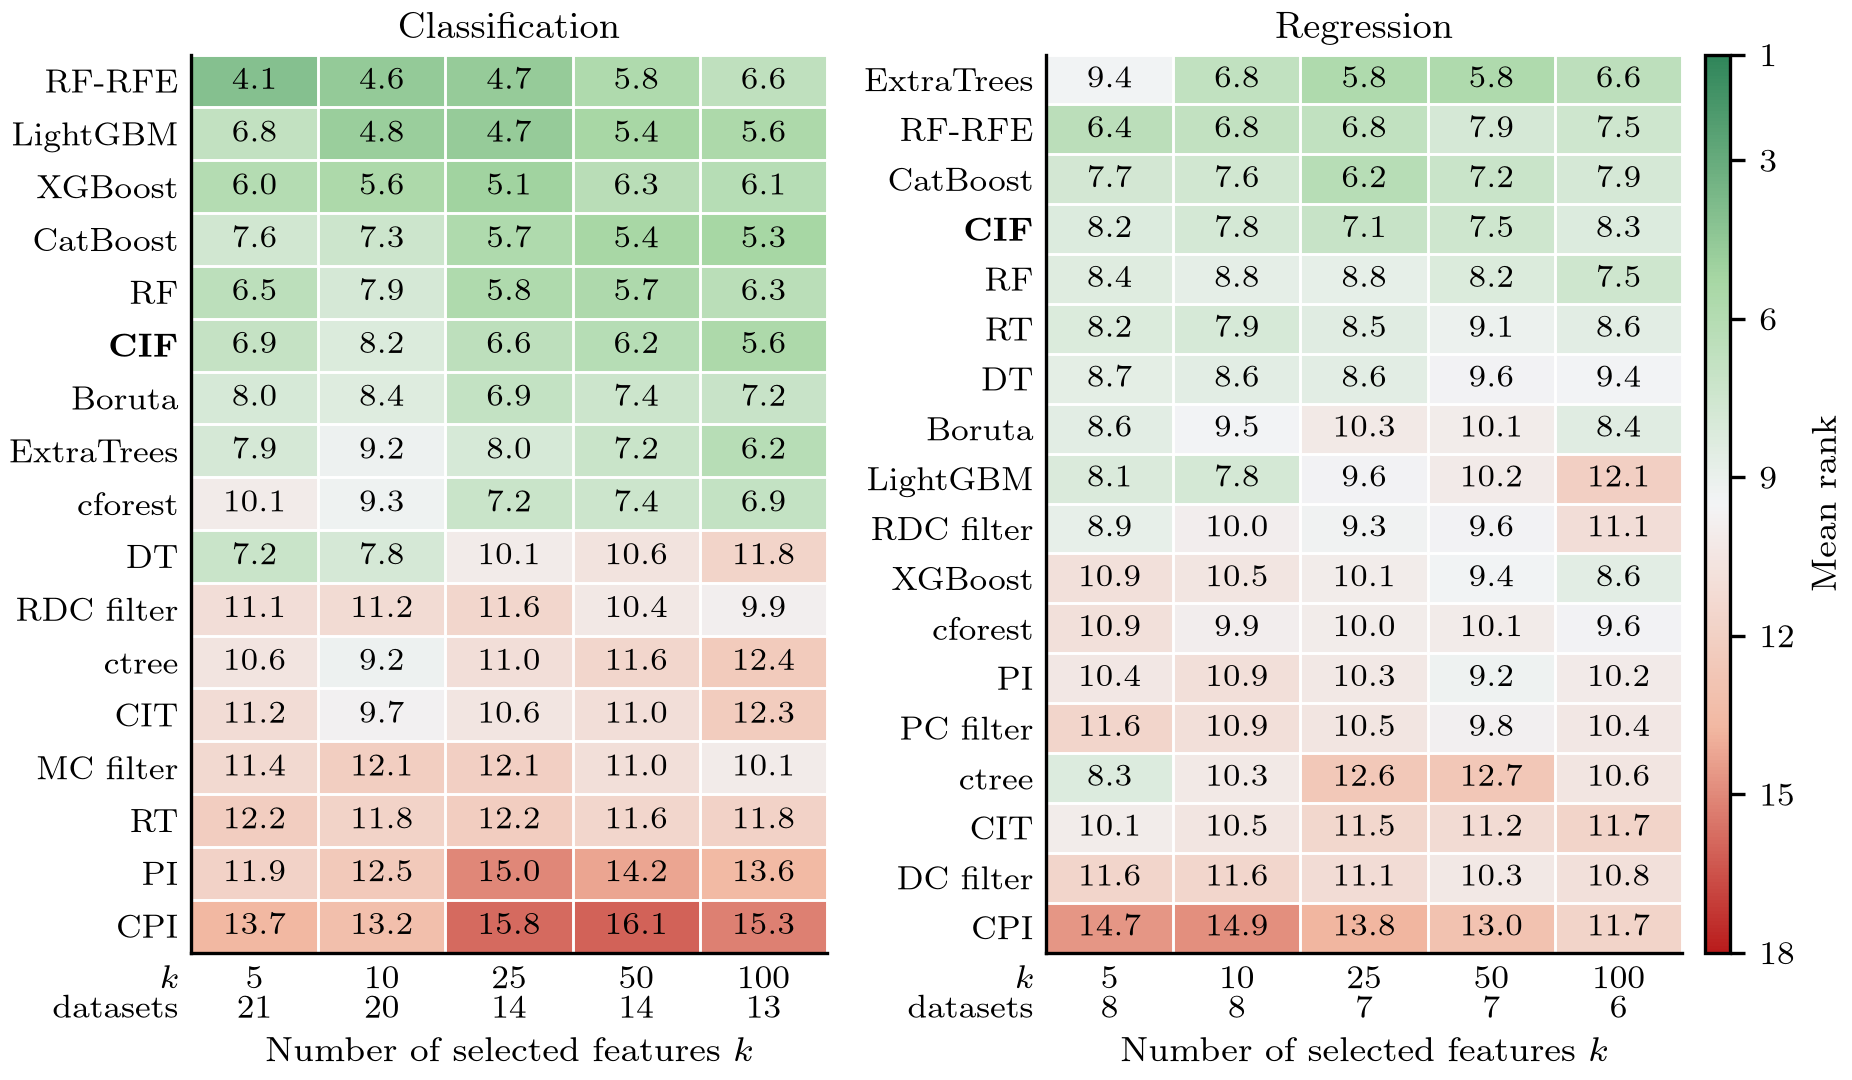
\includegraphics[width=0.95\linewidth]{figures/benchmark_k_trajectory.png}
  \caption{Mean rank of every feature selection method by the number of
  selected features $k$, for classification (left, 17 methods) and regression
  (right, 18 methods), averaged across downstream models at each value of $k$;
  lower ranks are better, and the two panels share one colour scale. Each
  column uses the datasets on which every method has results at that $k$, whose
  number is given under $k$.}
  \label{fig:k-trajectory}
\end{figure}

\paragraph{What the ranking rests on.}\label{sec:mechanism}

Of four targeted changes to the selected CIF configuration, only reducing the
forest to one tree lowers the score on every dataset, in both tasks
(\cref{tab:cif-ranking-ablation}). Split-count ranking, disabling bootstrap
sampling, and disabling feature muting change balanced accuracy by at most
0.001 on average, with intervals that include zero. In regression these three
changes lower the mean $R^2$, two of them with intervals that exclude zero, but
the three \nolinkurl{coepra} datasets set those means, and the medians stay
within 0.007 of zero.

\begin{table}[htb]
  \centering
  \footnotesize
  \setlength{\tabcolsep}{4pt}
  \renewcommand{\arraystretch}{1.08}
  \begin{tabular}{@{}llS[table-format=+1.3]S[table-format=+1.3]cc@{}}
    \toprule
    \tablehead{Task} & \tablehead{CIF change} & {Mean difference} & {Median difference} & 95\% interval & Wins--losses \\
    \midrule
    Classification & Split-count ranking & -0.001 & 0.000 & [$-$0.005, +0.002] & \winloss{12}{9} \\
    Classification & Disable bootstrap & -0.001 & 0.000 & [$-$0.004, +0.003] & \winloss{9}{12} \\
    Classification & Disable feature muting & +0.001 & 0.000 & [$-$0.001, +0.002] & \winloss{13}{5} \\
    Classification & Use one tree & -0.071 & -0.043 & [$-$0.101, $-$0.045] & \winloss{0}{22} \\
    \addlinespace
    Regression & Split-count ranking & -0.053 & -0.003 & [$-$0.142, $-$0.002] & \winloss{2}{6} \\
    Regression & Disable bootstrap & -0.064 & -0.007 & [$-$0.128, $-$0.010] & \winloss{4}{4} \\
    Regression & Disable feature muting & -0.157 & 0.000 & [$-$0.468, +0.001] & \winloss{4}{4} \\
    Regression & Use one tree & -0.658 & -0.059 & [$-$1.692, $-$0.054] & \winloss{0}{8} \\
    \bottomrule
  \end{tabular}
  \caption{CIF ablations on the real-data benchmark, 22 classification and 8
  regression datasets. Differences are the changed variant minus the selected
  CIF configuration in balanced accuracy or $R^2$, paired within seed and fold
  and averaged within each dataset over downstream learners, supported standard
  values of $k$, and the 25 paired replicates; positive values favor the
  variant. Intervals are percentile bootstrap intervals for the mean over
  datasets (20{,}000 replicates); wins and losses count datasets, with exact
  ties omitted.}
  \label{tab:cif-ranking-ablation}
\end{table}

\paragraph{Support.}
The support of a ranker is the set of features that win at least one split.
Features outside it tie at zero importance (\cref{sec:rank-construction}), so a
ranking carries information only within its support. On the synthetic datasets, random forests give every feature nonzero
importance on 15 of the 16 designs, and 800 of 1,000 on the 1,000-feature
classification design. On 13 of the 16 designs, CIF's support keeps 90 to
100\% of the planted features, so the support serves as a shortlist. A single
CIT splits on few features, so zero-importance filler makes up most of its
top-$k$ list: 52, 81, and 90\% of its top 10, 25, and 50 features, against 0,
3, and 14\% for CIF and none for random forests. This is consistent with CIT
ranking near the bottom of the benchmark.

\paragraph{Feature use in sampled forests.}
In sparse designs, feature sampling keeps informative features out of most CIF
splits (\cref{app:candidate-availability}). CIT, which considers every feature
at each node, uses informative features in 100.0\% of classification splits
and 93.5\% of regression splits. Over the 12 classification forest designs,
CIF uses them in 33.2\% of splits, against 91.7\% for CIF-all, 8.4\% for RF,
and 6.5\% for ExtraTrees. RF and ExtraTrees grow to purity, so most of their
splits are deep splits on noise, while CIF stops at the permutation test. With
32 of 1,000 features sampled at a node and two informative, an informative
feature is a candidate at 6.3\% of nodes, and when the sampled subset holds
none, Stage~A selects from the noise it was given.
